\documentclass[11pt]{article}
\usepackage{icmlko}
\begin{document}

\title{바닥 검사가 아홉 중 여섯에서 틀린 답을 줬다 --- 그리고 판에서 제일 높은 도메인은 위 0.36\%다}
\author{월드모델 실험실}
\date{노트 382 · 2026년 8월 1일}
\maketitle

\begin{abstract}
노트 381이 ``다른 도메인 균일 수집이 지금 제일 값이 크다''로 끝났다.
어느 도메인부터인지 정하려고 노트 375의 바닥 검사를 아홉 도메인에 돌렸다.
\textbf{검사가 틀렸다.}

노트 375는 \emph{최소$\div$1분위}가 1에 가까우면 절단이라 했다. 그것이
잡는 것은 \textbf{벽}(급격한 단절)이지 \textbf{바닥}(그냥 낮은 데서 멈춤)이
아니다. 라벨이 아래쪽에 자연스럽게 몰리는 도메인은 벽이 없어도 비가 1이
되고, 꼬리가 길면 한참 위에서 멈춰도 비가 0에 가깝다.

\textbf{고친 검사는 관측 최소를 그 라벨의 \emph{자연 바닥}과 견주는 것이다.}
아홉 라벨이 전부 셈꼴(관심 수 · 리뷰 수 · 후원자 수 · 판매지수)이라 자연
바닥은 1이다. 그러면 판정이 \textbf{아홉 중 여섯에서 뒤집힌다}:

\begin{center}
\begin{tabular}{lrr}
\hline
바닥까지 내려간다 & 애니 (1) · 모바일 (1) · 펀딩 (1) & --- \\
멈춰 있다 & 웹툰 19 · 게임 82 · 만화 633 · 아이돌 772 & \\
 & 도서 950 · 세계애니 19,533 & \\
\hline
\end{tabular}
\end{center}

\textbf{제일 큰 것을 걱정할 필요는 없었다.} 무게 711로 판에서 제일 무거운
웹툰은 수집이 네이버 웹툰 요일별 연재작 \emph{전부} $+$ 완결 아카이브라
사실상 전수조사다 --- 최소 19는 우리가 자른 게 아니라 플랫폼에 그보다
낮은 작품이 없는 것에 가깝다. \textbf{바닥이 있다고 다 우리 잘못은 아니다.}

\textbf{게임은 우리 잘못이고, 바닥이 둘이다.}
\texttt{game\_domain.top\_appids} 가 스팀 검색을 \texttt{filter=topsellers}
로 걸고 앞에서 600건을 받는데, \emph{같은 검색이 보고하는 전체가}
\textbf{167,368건}이다 --- 위 \textbf{0.36\%}. 그 위에 \texttt{build()} 가
``리뷰 총계 50 미만은 라벨이 못 된다''로 한 번 더 자른다. 남은 것이 482행.
\textbf{그리고 게임은 지금 판에서 제일 높은 도메인이다($+0.6040$).}

노트 379가 펀딩에서 같은 모양을 재니 도메인 점수가 4배 부풀어 있었다.
게임 균일 표본 2,000건을 모으는 중이다.
\end{abstract}

\section{검사가 왜 틀렸나}

노트 375가 수집 편향을 셋으로 나눴다 --- \emph{절단}(자연 바닥 위에 벽) ·
\emph{구역 편향}(바닥은 열렸는데 한 구역만 떴다) · \emph{열림}. 절단의
검사로 \textbf{최소$\div$1분위}를 썼다. 그 비가 1에 가까우면 최소 바로 위에
1\%가 몰려 있다는 뜻이고, 곧 벽이다.

\textbf{벽과 바닥은 다르다.} 두 가지로 어긋난다.

\textbf{첫째, 자연스러운 몰림을 벽으로 읽는다.} 펀딩 라벨은 후원자 수라
1명짜리 프로젝트가 2.2\%다. 최소도 1분위도 $\log_{10}1 = 0$ 이라 비가
정확히 1이 되고 검사는 ``절단''이라 답한다 --- \textbf{그런데 이 도메인은
바닥까지 내려가 있다.} 애니(리뷰 1건) · 모바일(평점 1건)도 같다.

\textbf{둘째, 긴 꼬리를 열림으로 읽는다.} 웹툰은 최소 19 · 1분위 474 라
비가 0.040 이고 검사는 ``열림''이라 답한다. 벽은 없다 --- 그런데
\emph{19에서 멈춘다.} 자연 바닥은 1이다.

\textbf{고침은 견주는 상대를 바꾸는 것이다} --- 1분위가 아니라 그 라벨이
가질 수 있는 제일 작은 값. 아홉 라벨이 전부 셈꼴이라 그 값은 1이다.

\begin{figure}[t]
\centering
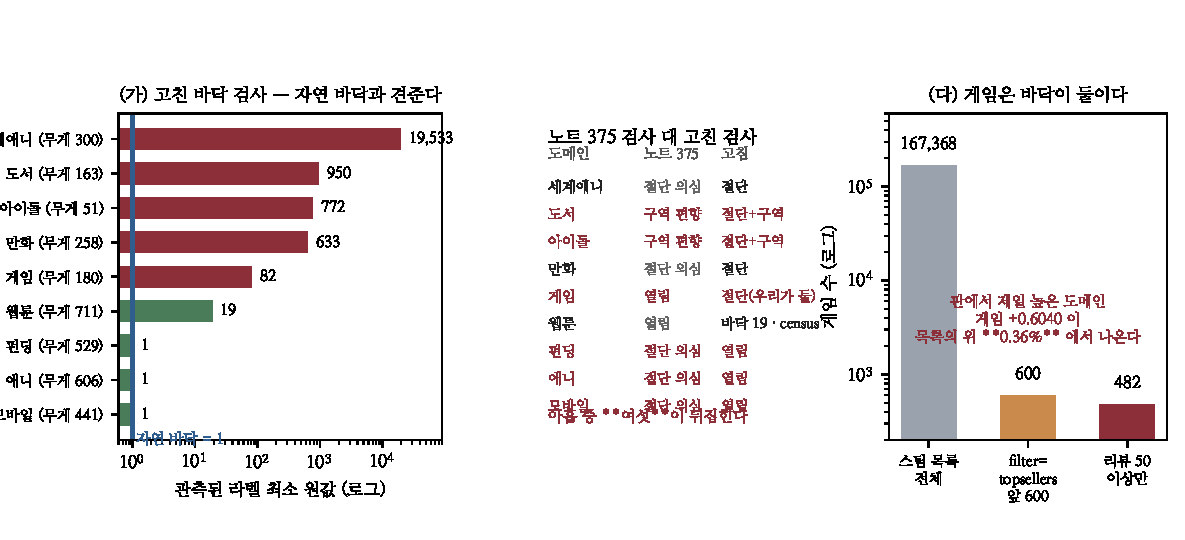
\includegraphics[width=\linewidth]{figs/fig382.pdf}
\caption{\textbf{(가)} 도메인별 관측 라벨 최소(원값, 로그축)와 자연 바닥 1.
초록 셋만 바닥에 닿는다. \textbf{(나)} 노트 375 판정과 고친 판정 ---
아홉 중 여섯이 뒤집힌다. \textbf{(다)} 게임의 바닥 둘. 스팀 검색이 보고하는
167,368건에서 \texttt{topsellers} 앞 600을 받고, 다시 리뷰 50 미만을 잘라
482행이 남는다.}
\label{fig:main}
\end{figure}

\section{바닥이 있다고 다 우리 잘못은 아니다}

멈춰 있는 여섯을 하나씩 열어 보면 두 종류다.

\textbf{모집단이 거기서 끝나는 것.} 웹툰 수집은
\texttt{titlelist/weekday}(요일별 연재작 전부)와
\texttt{titlelist/finished}(완결 아카이브, 갱신일 순 60쪽)다 --- 인기순으로
자른 데가 없다. 네이버 웹툰 정식 연재작에 관심 19 미만이 거의 없는 것은
우리 표본이 아니라 그 플랫폼의 성질이다. \textbf{무게 711로 제일 무거운
도메인이 여기 있는 것은 다행이다.}

\textbf{우리가 자른 것.} 게임이 그렇고, 아래에서 따로 본다. 도서는 이미
알려진 베스트셀러 스크랩이고(수집순$\leftrightarrow$라벨 $-0.4652$) 아이돌도
구역 편향이 같이 뜬다($+0.3513$). 만화 · 세계애니는 AniList 인기 순위
상위를 받은 것이라 파일이 라벨 순으로 \emph{정확히} 정렬돼 있다(수집순
상관 $-1.0000$) --- 그래서 이 둘에는 수집순 검사를 쓸 수 없다.
\textbf{정렬된 파일에서 수집순$\leftrightarrow$라벨은 표본이 아니라 정렬을
잰다.} 노트 375의 두 번째 검사도 조건이 붙는다.

세계애니는 노트 376이 이미 답했다 --- 바닥 아래를 받아 봤더니 신호가
$+0.0223$ 으로 없어서 안 넓혔다. \textbf{절단이 곧 고쳐야 할 것은
아니라는 반례가 이미 있다.}

\section{게임 --- 바닥이 둘이고 둘 다 우리 것이다}

\begin{center}
\begin{tabular}{lrl}
\hline
 & 게임 수 & 자른 것 \\
\hline
스팀 검색 전체 & 167,368 & --- \\
\texttt{filter=topsellers} 앞 600 & 600 & 위 \textbf{0.36\%} \\
\texttt{build()}: 리뷰 총계 $\ge 50$ & 482 & 반응 적은 것 \\
\hline
\end{tabular}
\end{center}

\textbf{두 선택 다 근거가 적혀 있다.} 원본 주석이 ``셔블웨어를 피하면서
연도 분포도 얻는 방법이다 --- 2024년 한 해에만 116,830개가 출시됐고
대부분은 반응 자체가 없다''고 쓰고, \texttt{build()} 는 ``반응이 거의
없는 것은 라벨이 못 된다''고 쓴다. \textbf{둘 다 말이 되는 이유고, 이
노트는 그것을 뒤집지 않는다.}

뒤집지 않는 대신 \textbf{크기를 잰다.} 노트 379가 펀딩에서 정확히 같은
모양 --- 목록이 정렬돼 있고 우리는 앞을 떴다 --- 을 재니 도메인 점수가
$+0.4195$ 에서 $+0.0866$ 으로 4.8배 부풀어 있었다. 게임은 지금 판에서
\textbf{제일 높은 도메인}($+0.6040$)이고 무게 180이다.

\textbf{셔블웨어를 모집단에 넣을지는 과제를 바꾸는 결정이라 점수로 정하지
않는다}(노트 224). 이 노트가 하는 것은 그 결정을 \emph{모르고} 내리지
않게 하는 것뿐이다 --- 지금은 아무도 정한 적 없이 기본값으로 되어 있다.

\texttt{ingest/game\_sample.py} 를 새로 썼다. 씨앗 고정(20260801)으로
목록 전체에서 쪽을 뽑고, \textbf{리뷰 50 문턱은 여기서 안 자른다} ---
두 바닥의 값을 따로 재려면 잘린 것도 받아 둬야 한다(\texttt{below\_old\_cut}
으로 표시만 한다). 2,000건 목표로 돌고 있다.

\section{남은 것}

\begin{center}
\begin{tabular}{lll}
\hline
항목 & 왜 값이 큰가 & 어떻게 \\
\hline
게임 균일 2,000 & 판 최고 도메인이 위 0.36\% 다 & 수집 중 · 노트 379 절차로 잰다 \\
리뷰 50 문턱 따로 & 바닥이 둘이라 값도 둘이다 & \texttt{below\_old\_cut} 으로 갈라 잰다 \\
도서 · 아이돌 & 절단 $+$ 구역이 겹친 둘 & 목록 구조부터 확인 \\
정렬된 파일의 수집순 & 만화 · 세계애니에 검사가 안 통한다 & 수집 시각 등 다른 순서를 찾는다 \\
\hline
\end{tabular}
\end{center}

\end{document}
